\documentclass[11pt,a4paper]{article}
\usepackage[utf8]{inputenc}
\usepackage[T1]{fontenc}
\usepackage[spanish,es-nodecimaldot]{babel}
\usepackage{lmodern}
\usepackage{geometry}
\geometry{margin=2.3cm}
\usepackage{amsmath,amssymb,mathtools}
\usepackage{siunitx}
\sisetup{output-decimal-marker={,},per-mode=symbol}
\usepackage{booktabs,tabularx,array}
\usepackage{graphicx}
\usepackage{float}
\usepackage{hyperref}
\usepackage{xcolor}
\usepackage{enumitem}
\usepackage{fancyhdr}
\usepackage{microtype}
\hypersetup{colorlinks=true,linkcolor=blue!50!black,urlcolor=blue!50!black}
\pagestyle{fancy}\fancyhf{}\lhead{Modelo de Pennes: diferencias finitas}\rhead{Desarrollo reproducible}\cfoot{\thepage}
\newcommand{\dd}{\mathrm{d}}
\newcommand{\OO}{\mathcal{O}}
\title{\vspace{-1cm}\textbf{Discretización por diferencias finitas de la ecuación de Pennes}\\[6pt]
\large Derivación con Taylor, condiciones de frontera, matriz tridiagonal y comparación con volúmenes finitos}
\author{Desarrollo didáctico y replicación independiente}
\date{22 de octubre de 2026}
\begin{document}
\maketitle
\begin{abstract}
Se desarrolla paso a paso un esquema de diferencias finitas para el problema de biotransferencia unidimensional examinado por Rojczyk y colaboradores (2015). Se deduce la fórmula centrada para la derivada segunda, se emplea Euler implícito para la derivada temporal y se tratan las condiciones de Dirichlet y Robin. Para mantener una matriz tridiagonal, la temperatura del nodo superficial se elimina algebraicamente usando aproximaciones de primer y segundo orden de la condición de Robin. Se reproducen las tres etapas físicas (estado estacionario, enfriamiento y recalentamiento) y se confrontan valores numéricos con una implementación independiente de volúmenes finitos. No se afirma replicar la implementación MATLAB ni la validación ANSYS originales.
\end{abstract}

\section{Problema físico, geometría e hipótesis}
El tejido se representa por una lámina homogénea de espesor $L=\SI{0.005}{\meter}$, con $x=0$ hacia el interior corporal y $x=L$ en la piel expuesta al ambiente. La temperatura es $T(x,t)$. Se adopta la ecuación de biocalor de Pennes, unidimensional, con propiedades constantes, perfusión sanguínea homogénea y producción metabólica volumétrica constante. La frontera interna se mantiene a temperatura arterial $T_a$, y la superficie externa intercambia calor mediante un coeficiente global $h$, que reúne convección y radiación linealizada. La temperatura corporal y la ambiental son constantes, y no se considera conducción lateral ni un tumor de geometría separada. Son las idealizaciones fundamentales del caso de estudio, no hipótesis clínicas comprobadas.

La ecuación es
\begin{equation}\label{eq:pennes}
 \rho c\frac{\partial T}{\partial t}
 =\frac{\partial}{\partial x}\left(k\frac{\partial T}{\partial x}\right)
 +\omega_b\rho_b c_b(T_a-T)+\dot q_m.
\end{equation}
Definimos
\begin{equation}\label{eq:abcd}
 A=\rho c,\qquad B=k,\qquad C=\omega_b\rho_b c_b,\qquad D=\dot q_m.
\end{equation}
Al ser $k=B$ constante,
\begin{equation}\boxed{A T_t=B T_{xx}+C(T_a-T)+D.}\label{eq:governing}\end{equation}
Cada término tiene unidades de $\mathrm{W\,m^{-3}}$. En particular $[A]=\mathrm{J\,m^{-3}\,K^{-1}}$, $[B]=\mathrm{W\,m^{-1}\,K^{-1}}$, $[C]=\mathrm{W\,m^{-3}\,K^{-1}}$ y $[D]=\mathrm{W\,m^{-3}}$.

\section{Las tres etapas físicas y las condiciones de frontera}
\subsection{Estado estacionario previo}
Antes del enfriamiento, se considera el perfil estacionario $T_{\mathrm{est}}(x)$ definido por
\begin{subequations}\label{eq:steady}
\begin{align}
 B T_{\mathrm{est}}''+C(T_a-T_{\mathrm{est}})+D&=0, &0<x<L,\\
 T_{\mathrm{est}}(0)&=T_a,\\
 -B T_{\mathrm{est}}'(L)&=h\bigl(T_{\mathrm{est}}(L)-T_\infty\bigr).
\end{align}
\end{subequations}
La última expresión proviene de igualar el flujo conductivo saliente $-B T_x$ con el flujo convectivo/radiativo $h(T_s-T_\infty)$. Puede escribirse $B T_x(L)+hT(L)=hT_\infty$.

\subsection{Enfriamiento previo: $-\SI{15}{\second}<t<0$}
La piel se coloca en contacto ideal con una reserva térmica a $T_c=\SI{0}{\celsius}$ durante $\SI{15}{\second}$. Se resuelve la ecuación \eqref{eq:governing} con las dos fronteras de Dirichlet:
\begin{equation}
T(0,t)=T_a,\qquad T(L,t)=T_c,\qquad
T(x,-15\,\mathrm{s})=T_{\mathrm{est}}(x).
\end{equation}
El perfil final $F(x)=T(x,0)$ sirve como condición inicial del recalentamiento. \textbf{No se impone $T_c=0$ durante el recalentamiento.}

\subsection{Recalentamiento: $0<t\le \SI{50}{\second}$}
Se retira la reserva fría y se restaura la frontera convectiva:
\begin{subequations}\label{eq:reheat}
\begin{align}
 A T_t &= B T_{xx}+C(T_a-T)+D,&&0<x<L,\\
 T(0,t)&=T_a,\\
 B T_x(L,t)+hT(L,t)&=hT_\infty,\\
 T(x,0)&=F(x).
\end{align}
\end{subequations}
El paso instantáneo entre la frontera $T(L,0)=T_c$ y la condición de Robin para $t>0$ puede generar una discontinuidad de compatibilidad en el punto $(L,0)$. El esquema implícito aplica la nueva condición a partir del primer paso de recalentamiento.

\section{Malla de diferencias finitas}
Sean $N$ intervalos espaciales de longitud $\Delta x=L/N$, de modo que existen $N+1$ nodos $x_i=i\Delta x$, $i=0,\dots,N$. Sean también $t_n=n\Delta t$ y $T_i^n\approx T(x_i,t_n)$. Se elige $N=27$ y $\Delta t=\SI{0.05}{\second}$ para el experimento de comparación. Así,
\begin{equation}
\Delta x=\frac{0.005}{27}=1.85185185\times10^{-4}\ \mathrm m.
\end{equation}
\textit{Importante:} 27 intervalos finitos producen 28 nodos. Los 27 \emph{volúmenes} del artículo original no son idénticos a 27 intervalos MDF, aunque ambos emplean el mismo $\Delta x$.

\section{Derivación de la segunda derivada espacial por Taylor}
Se desarrollan las temperaturas a ambos lados del nodo $i$ en torno a $x_i$, a un tiempo fijo:
\begin{align}
T(x_i+\Delta x,t)&=T_i+\Delta x T_x+\frac{\Delta x^2}{2}T_{xx}+\frac{\Delta x^3}{6}T_{xxx}+\frac{\Delta x^4}{24}T_{xxxx}+\OO(\Delta x^5),\\
T(x_i-\Delta x,t)&=T_i-\Delta x T_x+\frac{\Delta x^2}{2}T_{xx}-\frac{\Delta x^3}{6}T_{xxx}+\frac{\Delta x^4}{24}T_{xxxx}+\OO(\Delta x^5).
\end{align}
Al sumar, los términos impares se cancelan:
\begin{equation}
T_{i+1}+T_{i-1}-2T_i=\Delta x^2T_{xx}+\frac{\Delta x^4}{12}T_{xxxx}+\OO(\Delta x^6).
\end{equation}
Por lo tanto,
\begin{equation}\boxed{T_{xx}(x_i,t)=\frac{T_{i+1}-2T_i+T_{i-1}}{\Delta x^2}+\OO(\Delta x^2).}\label{eq:xx}\end{equation}
La aproximación tiene orden espacial dos en los nodos interiores para una solución suficientemente regular.

\section{Derivación de la primera derivada temporal}
La expansión hacia atrás desde $t_{n+1}$ es
\begin{equation}
T(x_i,t_n)=T_i^{n+1}-\Delta t\,T_t(x_i,t_{n+1})+\frac{\Delta t^2}{2}T_{tt}(x_i,t_{n+1})+\OO(\Delta t^3).
\end{equation}
Al despejar,
\begin{equation}\boxed{T_t(x_i,t_{n+1})=\frac{T_i^{n+1}-T_i^n}{\Delta t}+\OO(\Delta t).}\label{eq:tt}\end{equation}
Esta es la fórmula de Euler hacia atrás. A diferencia de Euler explícito, todos los términos físicos que dependen de $T$ se evalúan en el tiempo nuevo $n+1$.

\section{Ecuación discreta interior y agrupación}
Sustituimos \eqref{eq:xx} y \eqref{eq:tt} en \eqref{eq:governing}:
\begin{equation}
A\frac{T_i^{n+1}-T_i^n}{\Delta t}=B\frac{T_{i-1}^{n+1}-2T_i^{n+1}+T_{i+1}^{n+1}}{\Delta x^2}+C(T_a-T_i^{n+1})+D.
\end{equation}
Pasamos las incógnitas del nuevo paso al lado izquierdo:
\begin{equation}\label{eq:row}
-\frac{B}{\Delta x^2}T_{i-1}^{n+1}+
\left(\frac{A}{\Delta t}+\frac{2B}{\Delta x^2}+C\right)T_i^{n+1}
-\frac{B}{\Delta x^2}T_{i+1}^{n+1}
=\frac{A}{\Delta t}T_i^n+CT_a+D.
\end{equation}
Definimos para acortar:
\begin{equation}\label{eq:defs}
 a=\frac A{\Delta t},\qquad r=\frac B{\Delta x^2},\qquad s=a+2r+C,\qquad f=CT_a+D.
\end{equation}
Entonces, para los nodos $i=1,\ldots,N-1$,
\begin{equation}\boxed{-rT_{i-1}^{n+1}+sT_i^{n+1}-rT_{i+1}^{n+1}=aT_i^n+f.}\label{eq:interior}\end{equation}
En particular, al usar la temperatura interior conocida $T_0^{n+1}=T_a$, la primera ecuación es
\begin{equation}\label{eq:first}
sT_1^{n+1}-rT_2^{n+1}=aT_1^n+f+rT_a.
\end{equation}

\section{Frontera derecha de Dirichlet durante el enfriamiento}
Durante el contacto con la reserva fría, $T_N^{n+1}=T_c=0$. La última ecuación interior se vuelve
\begin{equation}\label{eq:cool}
-rT_{N-2}^{n+1}+sT_{N-1}^{n+1}=aT_{N-1}^n+f+rT_c.
\end{equation}
Por eso, la matriz de coeficientes durante el enfriamiento para el vector de incógnitas $\boldsymbol u=(T_1,\dots,T_{N-1})^\mathsf T$ es
\begin{equation}\label{eq:mcool}
\underbrace{\begin{pmatrix}
s&-r&0&\cdots&0\\
-r&s&-r&\ddots&\vdots\\
0&\ddots&\ddots&\ddots&0\\
\vdots&\ddots&-r&s&-r\\
0&\cdots&0&-r&s
\end{pmatrix}}_{M_{\mathrm{frio}}}
\boldsymbol u^{n+1}=
 a\boldsymbol u^n+f\boldsymbol 1+rT_a\boldsymbol e_1+rT_c\boldsymbol e_{N-1}.
\end{equation}
En esta ecuación $T_c=0$, pero se conserva el término para mostrar de dónde procede. Para calcular el estado estacionario se utiliza la matriz correspondiente a la etapa con Robin, pero se toma $a=0$.

\section{Condición de Robin en la superficie durante el recalentamiento}
El flujo conductivo superficial saliente es
\begin{equation}-B\left.\frac{\partial T}{\partial x}\right|_{L}=h(T_N-T_\infty).\end{equation}
Su tratamiento numérico exige atención: la derivada se evalúa en una frontera y no dispone de un nodo exterior físico.

\subsection{Opción 1: diferencia hacia atrás de primer orden}
Taylor alrededor de $x_N$ produce
\begin{equation}
T_{N-1}=T_N-\Delta x T_x(L)+\frac{\Delta x^2}{2}T_{xx}(L)+\cdots,
\end{equation}
de modo que
\begin{equation}\label{eq:robin1}
 B\frac{T_N^{n+1}-T_{N-1}^{n+1}}{\Delta x}+hT_N^{n+1}=hT_\infty,\qquad \text{error }\OO(\Delta x).
\end{equation}
Definimos $K_1=B/\Delta x$ y $H_1=h+K_1$. Despejamos la temperatura de superficie:
\begin{equation}\boxed{T_N^{n+1}=\frac{hT_\infty+K_1T_{N-1}^{n+1}}{H_1}.}\label{eq:tn1}\end{equation}
Al sustituirla en \eqref{eq:interior} con $i=N-1$:
\begin{equation}\label{eq:last1}
-rT_{N-2}^{n+1}+
\left(s-\frac{rK_1}{H_1}\right)T_{N-1}^{n+1}
=aT_{N-1}^n+f+\frac{rhT_\infty}{H_1}.
\end{equation}
La matriz de las incógnitas interiores permanece tridiagonal, pero la frontera solo está aproximada con orden uno.

\subsection{Opción 2 (recomendada): diferencia hacia atrás de segundo orden}
Consideremos ahora tres nodos $x_N$, $x_{N-1}$ y $x_{N-2}$. Sus expansiones son
\begin{align}
T_{N-1}&=T_N-\Delta x T_x+\frac{\Delta x^2}{2}T_{xx}-\frac{\Delta x^3}{6}T_{xxx}+\OO(\Delta x^4),\\
T_{N-2}&=T_N-2\Delta x T_x+2\Delta x^2T_{xx}-\frac{4}{3}\Delta x^3T_{xxx}+\OO(\Delta x^4).
\end{align}
Restamos cuatro veces la primera expansión y sumamos tres veces $T_N$:
\begin{equation}
3T_N-4T_{N-1}+T_{N-2}=2\Delta x T_x(L)+\OO(\Delta x^3).
\end{equation}
Así,
\begin{equation}\label{eq:robin2}
B\frac{3T_N^{n+1}-4T_{N-1}^{n+1}+T_{N-2}^{n+1}}{2\Delta x}
+hT_N^{n+1}=hT_\infty,
\end{equation}
con truncamiento de orden $\OO(\Delta x^2)$ en la derivada de la frontera. Sea $K_2=B/(2\Delta x)$, $H_2=h+3K_2$. Podemos despejar
\begin{equation}\boxed{T_N^{n+1}=\frac{hT_\infty+4K_2T_{N-1}^{n+1}-K_2T_{N-2}^{n+1}}{H_2}.}\label{eq:tn2}\end{equation}
Sustituimos \eqref{eq:tn2} en la ecuación del último nodo interior:
\begin{align}
-rT_{N-2}^{n+1}+sT_{N-1}^{n+1}
-r\frac{hT_\infty+4K_2T_{N-1}^{n+1}-K_2T_{N-2}^{n+1}}{H_2}
&=aT_{N-1}^n+f.
\end{align}
Agrupamos términos:
\begin{equation}\boxed{
\left(-r+\frac{rK_2}{H_2}\right)T_{N-2}^{n+1}
+\left(s-\frac{4rK_2}{H_2}\right)T_{N-1}^{n+1}
=aT_{N-1}^n+f+\frac{rhT_\infty}{H_2}.}
\label{eq:last2}
\end{equation}
Nótese que la incorporación directa de la fórmula de tres puntos en una fila independiente de Robin introduce un coeficiente en la segunda subdiagonal. \textbf{La eliminación algebraica de $T_N$ evita ese ensanchamiento de banda} y permite resolver exclusivamente los $N-1$ nodos interiores mediante una matriz tridiagonal.

\section{Sistema matricial tridiagonal durante el recalentamiento}
Para la aproximación Robin de segundo orden, llamemos
\begin{equation}
\ell_*=-r+\frac{rK_2}{H_2},\qquad d_*=s-\frac{4rK_2}{H_2},\qquad b_*=aT_{N-1}^n+f+\frac{rhT_\infty}{H_2}.
\end{equation}
Entonces,
\begin{equation}\label{eq:matrix}
\underbrace{\begin{pmatrix}
s&-r&0&\cdots&0\\
-r&s&-r&\ddots&\vdots\\
0&\ddots&\ddots&\ddots&0\\
\vdots&\ddots&-r&s&-r\\
0&\cdots&0&\ell_*&d_*
\end{pmatrix}}_{M_{\mathrm{Robin},2}}
\underbrace{\begin{pmatrix}T_1^{n+1}\\T_2^{n+1}\\\vdots\\T_{N-2}^{n+1}\\T_{N-1}^{n+1}\end{pmatrix}}_{\boldsymbol u^{n+1}}
=\underbrace{\begin{pmatrix}
aT_1^n+f+rT_a\\aT_2^n+f\\\vdots\\aT_{N-2}^n+f\\b_*
\end{pmatrix}}_{\boldsymbol b^{n+1}}.
\end{equation}
Resuelto $\boldsymbol u^{n+1}$, recuperamos $T_N^{n+1}$ mediante \eqref{eq:tn2}, mientras que $T_0^{n+1}=T_a$. La matriz no es simétrica debido a la modificación de la última fila, pero sigue siendo tridiagonal.

\section{Estado estacionario por el mismo sistema numérico}
En estado estacionario $T_t=0$. Por consiguiente, se usa $a=0$ y $s=2r+C$ en las ecuaciones \eqref{eq:first}, \eqref{eq:interior} y \eqref{eq:last2}, con $T_N$ recuperado por \eqref{eq:tn2}. No es correcto utilizar la ecuación transitoria con un paso de tiempo grande para definir sin más la condición inicial: el estado estacionario se determina resolviendo el sistema algebraico sin término de acumulación.

Como comprobación independiente también puede resolverse analíticamente
\begin{equation}
BT''-CT+CT_a+D=0.
\end{equation}
Para $C>0$, $\lambda=\sqrt{C/B}$ y $T_p=T_a+D/C$, de donde
\begin{equation}
T_{\mathrm{est}}(x)=T_p+E\cosh(\lambda x)+F_0\sinh(\lambda x),\qquad E=T_a-T_p=-D/C.
\end{equation}
La condición de Robin permite obtener
\begin{equation}
F_0=\frac{-h(T_p-T_\infty)-E\bigl[B\lambda\sinh(\lambda L)+h\cosh(\lambda L)\bigr]}{B\lambda\cosh(\lambda L)+h\sinh(\lambda L)}.
\end{equation}
Este perfil analítico es útil para validar la discretización estacionaria por refinamiento de malla, aunque el código anexo utiliza la solución estacionaria discreta de cada método para iniciar el enfriamiento.

\section{Parámetros del artículo y número de pasos}
\begin{table}[H]\centering\small
\begin{tabular}{lll}\toprule
Cantidad & Tejido sano & Tejido tumoral\\\midrule
$L$ [m] & 0.005 & 0.005\\
$T_a$ [$^\circ$C] & 37 & 37\\
$T_\infty$ [$^\circ$C] & 23 & 23\\
$h$ [W/(m$^2$ K)] & 10 & 10\\
$\rho$ [kg/m$^3$] & 1085 & 1085\\
$c$ [J/(kg K)] & 3680 & 3680\\
$B=k$ [W/(m K)] & 0.47 & 0.47\\
$\rho_b$ [kg/m$^3$] & 1060 & 1060\\
$c_b$ [J/(kg K)] & 3617 & 3617\\
$\omega_b$ [s$^{-1}$] & 0.00105 & 0.00525\\
$D$ [W/m$^3$] & 631 & 6310\\\bottomrule
\end{tabular}
\caption{Valores nominales de la tabla 1 de Rojczyk et al. (2015).}
\end{table}
Los parámetros agrupados resultan
\begin{equation}
A=1085(3680)=3\,992\,800\ \mathrm{J\,m^{-3}\,K^{-1}},\qquad
C_{\mathrm{sano}}=4025.721,\quad C_{\mathrm{tumoral}}=20128.605\ \mathrm{W\,m^{-3}\,K^{-1}}.
\end{equation}
Con $\Delta t=0.05$ s se necesitan $15/0.05=300$ pasos de enfriamiento y $50/0.05=1000$ pasos de recalentamiento. La temperatura superficial simulada se toma como $T_N^n$ en MDF, y como la reconstrucción de la temperatura de pared en MVF.

\section{Comparación rigurosa con volúmenes finitos}
\subsection{Ecuación de balance de un volumen interior}
En MVF no se discretiza directamente $T_{xx}$, sino que se integra el balance sobre un volumen $V_j$ de longitud $\Delta x$ y sección $S$. El volumen tiene un centro de temperatura $\bar T_j$ y dos caras. El balance es
\begin{equation}
A S\Delta x\frac{\bar T_j^{n+1}-\bar T_j^n}{\Delta t}
= S\bigl[q_{j-1/2}^{n+1}-q_{j+1/2}^{n+1}\bigr]
+ S\Delta x\bigl[C(T_a-\bar T_j^{n+1})+D\bigr],
\end{equation}
donde los flujos conducidos entre centros se aproximan por $q_{j+1/2}=-B(\bar T_{j+1}-\bar T_j)/\Delta x$. En un volumen interior, después de dividir por $S\Delta x$, se obtiene la misma forma algebraica que \eqref{eq:interior}. \textbf{Coincidencia algebraica interior no equivale a igualdad de método ni de ubicación de incógnitas.}

\subsection{Frontera superficial en MVF}
El último centro volumétrico está situado a $\Delta x/2$ de la pared. La conducción desde el centro hasta la pared y la convección exterior actúan como resistencias térmicas en serie. Así,
\begin{equation}\label{eq:heff}
 h_{\mathrm{ef}}=\left(\frac{\Delta x}{2B}+\frac{1}{h}\right)^{-1}.
\end{equation}
En la ecuación del último volumen aparece la contribución $h_{\mathrm{ef}}(T_\infty-\bar T_{N-1})/\Delta x$. Su temperatura de pared se calcula como
\begin{equation}\label{eq:wall}
T_s=\frac{(2B/\Delta x)\,\bar T_{N-1}+hT_\infty}{2B/\Delta x+h}.
\end{equation}
El primer volumen se comunica con la frontera interna fija mediante una distancia $\Delta x/2$, que produce un coeficiente conductivo $2B/\Delta x^2$ en la ecuación dividida por volumen.

\subsection{Resultados calculados de manera independiente}
Se calcularon soluciones para tejido sano y tumoral con $N=27$ y $\Delta t=0.05$ s. Los resultados son \textit{simulaciones de la reimplementación independiente}, no valores que se atribuyan a las tablas originales.
\begin{table}[H]\centering\small
\begin{tabular}{llrrrr}\toprule
Tejido & Tiempo [s] & MDF Robin 1 [$^\circ$C] & MDF Robin 2 [$^\circ$C] & MVF [$^\circ$C] & MDF2--MVF [K]\\\midrule
Sano & 1 & 7.5729 & 6.3830 & 6.1741 & 0.2089\\
Sano & 10 & 17.5307 & 16.5421 & 16.4735 & 0.0687\\
Sano & 50 & 26.9682 & 26.3713 & 26.3451 & 0.0263\\
Tumoral & 1 & 8.0258 & 6.8037 & 6.5834 & 0.2203\\
Tumoral & 10 & 18.7029 & 17.7453 & 17.6760 & 0.0694\\
Tumoral & 50 & 28.9581 & 28.4781 & 28.4556 & 0.0224\\\bottomrule
\end{tabular}
\caption{Comparación numérica con datos y condiciones del artículo. Las diferencias se calculan entre soluciones discretas.}
\end{table}
\begin{figure}[H]\centering
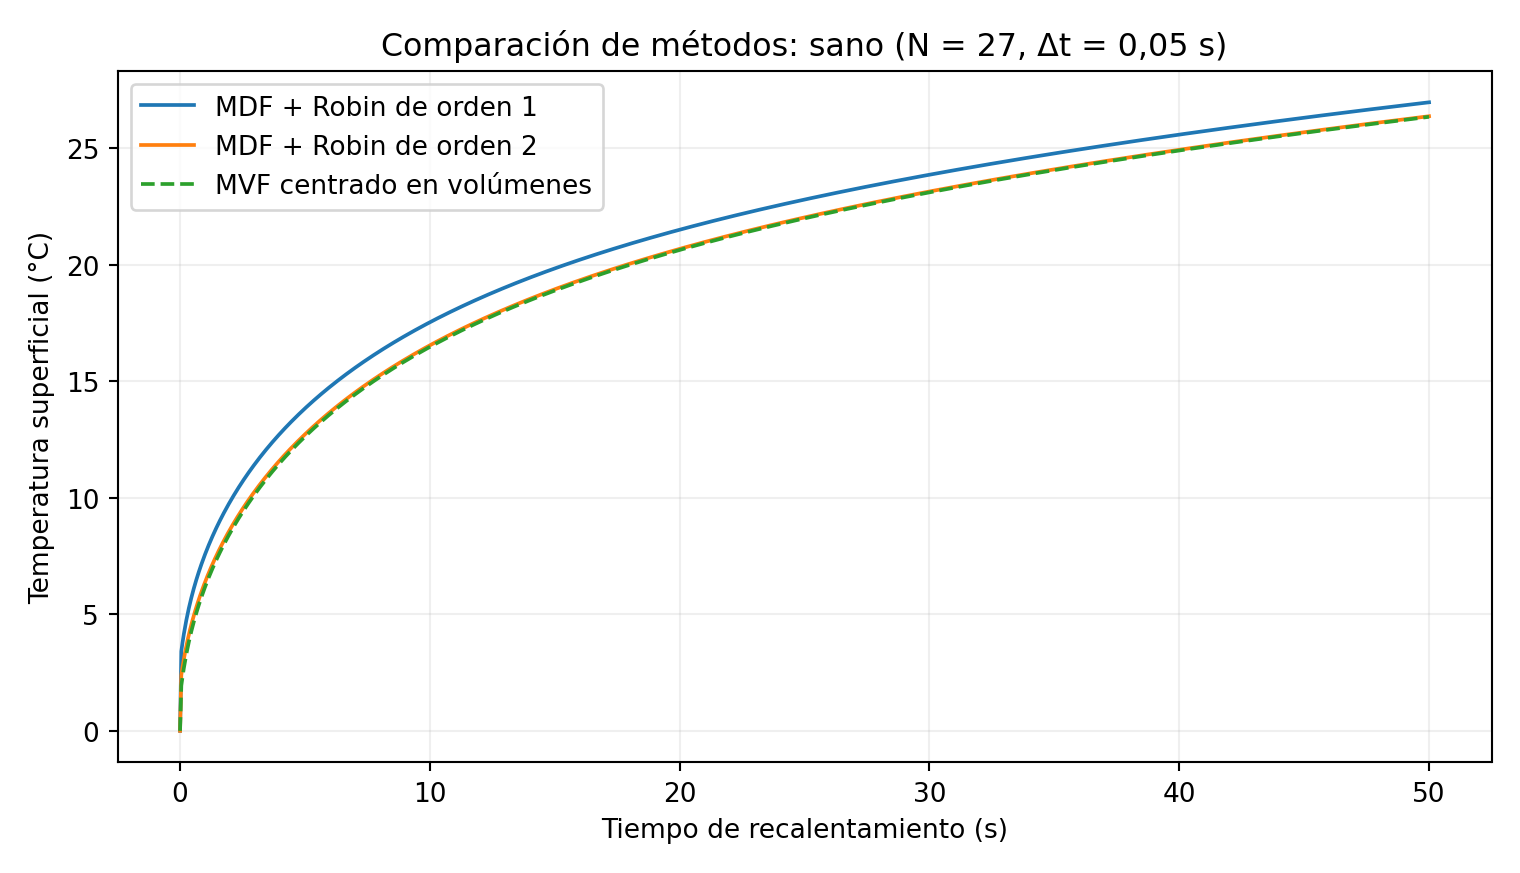
\includegraphics[width=0.93\linewidth]{comparacion_sano.png}
\caption{Evolución superficial calculada para tejido sano.}
\end{figure}
\begin{figure}[H]\centering
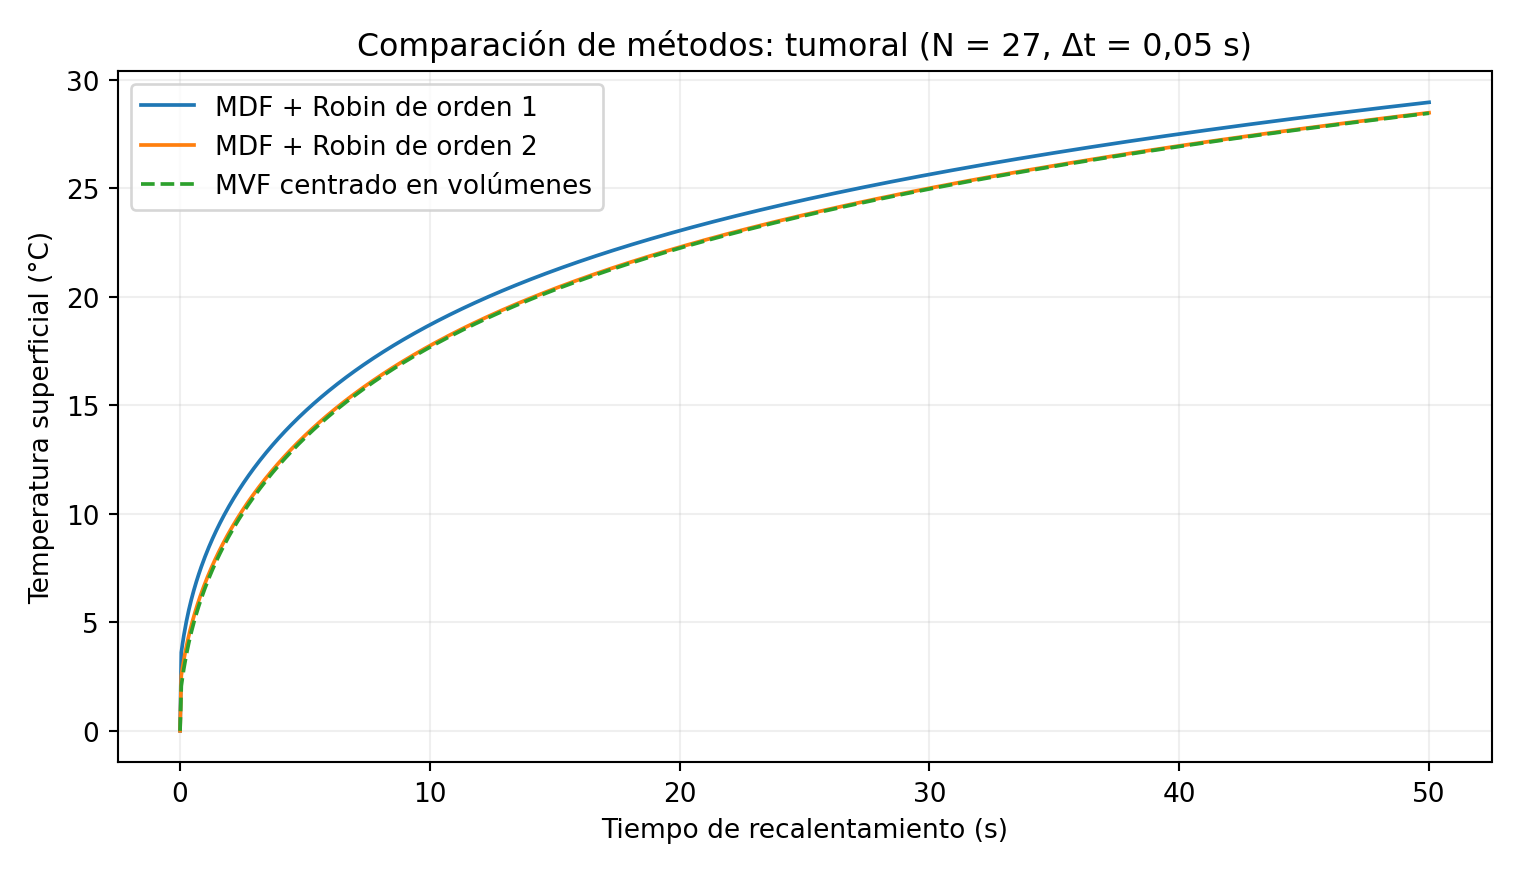
\includegraphics[width=0.93\linewidth]{comparacion_tumoral.png}
\caption{Evolución superficial calculada para tejido tumoral.}
\end{figure}
\subsection{Verificación con refinamiento}
Para el recalentamiento a $t=50$ s:
\begin{table}[H]\centering\small
\begin{tabular}{lrrrr}\toprule
Tejido & $N$ & MDF Robin 1 [$^\circ$C] & MDF Robin 2 [$^\circ$C] & MVF [$^\circ$C]\\\midrule
Sano & 27 & 26.96824 & 26.37134 & 26.34505\\
Sano & 54 & 26.65095 & 26.34059 & 26.33406\\
Sano &108 & 26.49107 & 26.33294 & 26.33131\\
Tumoral &27 & 28.95813 & 28.47805 & 28.45563\\
Tumoral &54 & 28.70218 & 28.45180 & 28.44619\\
Tumoral &108 & 28.57301 & 28.44523 & 28.44383\\\bottomrule
\end{tabular}
\caption{Refinamiento espacial manteniendo $\Delta t=0.05$ s.}
\end{table}
Por ejemplo, en tejido sano la diferencia MDF2--MVF a $t=50$ s desciende de $0.02628$ K ($N=27$) a $0.00653$ K ($N=54$) y $0.00163$ K ($N=108$). Esta reducción, próxima a un factor cuatro por duplicación de $N$, es compatible con convergencia espacial de orden dos en esa diferencia. \textbf{No representa por sí sola una demostración del error absoluto} de cada método, ni prueba equivalencia con la implementación de los autores, y las discrepancias temporales comunes se mantienen porque $\Delta t$ es fijo.

\section{Algoritmo de resolución y uso del código}
\begin{enumerate}[label=\arabic*.]
\item Asignar $A,B,C,D,L,T_a,T_\infty,h,N,\Delta t$ y escoger el caso sano o tumoral.
\item Construir $r=B/\Delta x^2$ y la matriz estacionaria con $a=0$ y frontera Robin.
\item Resolver el estado estacionario y retener sus temperaturas interiores.
\item Cambiar la condición de superficie a Dirichlet $T_c=0$; construir una vez la matriz implícita de enfriamiento.
\item Ejecutar 300 pasos de enfriamiento, resolviendo un sistema tridiagonal por paso.
\item Restaurar la condición Robin de segundo orden; construir una vez la matriz implícita de recalentamiento.
\item Ejecutar 1000 pasos, registrar $T_N$ y repetir para ambos tejidos.
\item Ejecutar también MDF Robin de primer orden y MVF de centros de volumen, comparando las tres curvas y refinando $N$.
\end{enumerate}
La implementación de referencia provista en el archivo \texttt{comparar\_mdf\_mvf.py} resuelve las matrices tridiagonales mediante el algoritmo de Thomas sin depender de un solucionador externo; emplea \texttt{numpy} y \texttt{matplotlib} para arreglos y gráficos. Desde la carpeta del proyecto se ejecuta:
\begin{center}\texttt{python comparar\_mdf\_mvf.py}\end{center}
Se generan \texttt{comparacion\_sano.png}, \texttt{comparacion\_tumoral.png} y \texttt{comparacion\_mdf\_mvf.csv}.

\section{Alcance y limitaciones}
La deducción mediante Taylor y el esquema MDF son extensiones metodológicas para estudio y verificación; \textbf{el artículo no utiliza esta misma discretización por diferencias finitas}. Los autores publicaron un método implícito de volúmenes finitos con diferencias centrales, 27 volúmenes y $\Delta t=0.05$ s; la solución directa fue contrastada con ANSYS. Aquí no se dispone de su código MATLAB, las matrices exactas empleadas ni sus resultados numéricos punto a punto, y por ello no se puede afirmar igualdad con su simulación. Las magnitudes presentadas describen dos escenarios sintéticos y no constituyen precisión diagnóstica clínica.

\begin{thebibliography}{9}
\bibitem{rojczyk} M. Rojczyk, H. R. B. Orlande, M. J. Colaço, I. Szczygieł, A. J. Nowak, R. A. Białecki y Z. Ostrowski, ``Inverse heat transfer problems: an application to bioheat transfer,'' \textit{Computer Assisted Methods in Engineering and Science}, vol. 22, pp. 365--383, 2015. Documento proporcionado para esta replicación, especialmente las ecuaciones (17)--(21) y tablas 1--2.
\end{thebibliography}
\end{document}
